% ---------------------------------------------------------------------------
% HBNN anomaly-aware results. Paste into "Results and Analysis", e.g. after
% "Ablation Analysis" and before "Discussion". Needs: booktabs, graphicx.
% Figure files: hbnn_fig_accuracy.pdf, hbnn_fig_ratio.pdf, hbnn_fig_service.pdf, hbnn_fig_spike.pdf
% ---------------------------------------------------------------------------
\subsection{Anomaly-Aware HBNN}
\label{sec:hbnn_results}

The ablation above uses a point forecaster. To see whether the anomaly inputs also matter for a probabilistic model, we trained the HBNN with and without them on the same eleven traces. The setup differs from the LSTM study in a few ways that matter when reading the numbers. In the anomaly-aware variant each resource is given its workload channel together with its binary flag and its severity score, so a univariate model sees three channels and a bivariate model six. The loss is the Gaussian negative log-likelihood, so there is no asymmetric or spike weighting here. Windows were split chronologically by target time into 64\% training, 16\% validation and 20\% test. One hyperparameter set, taken from the reference M-B configuration (a convolution with 16 filters of width 3, an LSTM with 32 units, two dense layers of 32 units and a Bayesian dense layer with 8 units), was used for all four configurations, and no hyperparameter search was run. Four configurations, two input variants, eleven traces and three seeds give 216 fits. Predictive uncertainty comes from 100 stochastic forward passes: the aleatoric part is the mean predicted variance, the epistemic part is the variance of the predicted means across passes, and the upper bound at target level $\gamma$ is the mean plus $z_\gamma$ times the square root of the total variance. Because of these differences the raw HBNN numbers below are not an exact reproduction of~\cite{rossi2025}, and they should not be compared directly with the LSTM results.

\textit{Point accuracy.}
Table~\ref{tab:hbnn_acc} and Fig.~\ref{fig:hbnn_acc} give the point-forecast results. In the multi-trace configurations the anomaly inputs lower the CPU MSE from 0.0198 to 0.0031 for both M-U and M-B, and the memory MSE of M-B from 0.0179 to 0.0031. M-U memory is the exception: the two variants are indistinguishable at 0.0029. For the single-trace configurations the picture is mixed. S-B improves by about 20--23\% in MSE, while S-U is unchanged for CPU and about 11\% lower for memory. The paired ratios in Fig.~\ref{fig:hbnn_ratio} tell the same story, but the error bars of the single-trace models are wide (for example an MSE ratio of 1.43 for S-U CPU with a standard error of about 0.3), so we do not read those as a consistent gain or loss.

We are careful with the large gains of the multi-trace models. The raw M-U CPU and M-B models vary a lot between runs (an MSE standard deviation of 0.0276 around a mean of 0.0198), while the raw M-U memory model, trained in the same way, reaches 0.0029. This suggests that part of the gap comes from unstable training of the raw models and not from the anomaly inputs alone. We did not check run by run which fits drive it, so the safest statement is that the anomaly-aware multi-trace models were both more accurate and much more consistent in this experiment.

\textit{Spikes.}
Fig.~\ref{fig:hbnn_spike}(a,b) and the right half of Table~\ref{tab:hbnn_acc} look at the spike points. Spike MSE falls by 55--62\% for the multi-trace models (again except M-U memory), for instance from 0.0225 to 0.0102 for M-B CPU. At the same time the share of spike points where the mean forecast lies below the actual demand rises from about 90\% to 98--99\% in those cases. The network gets closer to the spike but almost always still lands under it. This is the behaviour the asymmetric, spike-weighted loss was designed to correct, and with a plain negative log-likelihood the anomaly inputs alone do not.

\textit{Service level.}
Table~\ref{tab:hbnn_service} and Fig.~\ref{fig:hbnn_service} show what an operator would see when choosing a target level. For M-B, the anomaly-aware model reaches an SR of 95.8\% at the 95\% target with a TPR of 116\%, whereas the raw model reaches 93.7\% with 129\%. At the 99\% target both realise about 98.5\%, but the raw model provisions 142.5\% of the demand against 123.0\%. The mean calibration gap falls from 3.7 to 2.2 percentage points for M-B and from 2.9 to 1.9 for M-U. The single-trace models behave differently. The upper bound is much looser and the anomaly inputs make no consistent difference: S-B needs 151--156\% of the demand at the 95\% target, and S-U already reaches an SR of about 98\% at the 90\% target while provisioning roughly twice the demand, which means its predicted variance is far too large. The S-U error is also well above the published value (an MSE of about 0.06 against 0.0047 in~\cite{rossi2025}). We read this as a sign that one shared hyperparameter set does not suit models trained on a single trace, and not as a property of the HBNN itself.

\textit{Uncertainty and cost.}
Aleatoric variance dominates throughout (Fig.~\ref{fig:hbnn_spike}c). The epistemic part is below 6\% of the total variance for the multi-trace models and 13--26\% for the single-trace ones, which have less data to learn from. The epistemic share is higher with the anomaly inputs mostly because the aleatoric variance of the raw multi-trace models is several times larger, not because the epistemic variance grows much. The extra input channels cost little: training time rises from 601 s to 807 s for M-B (the anomaly-aware runs trained for more epochs) and by about 15 s for S-B, with no change for S-U, and inference takes 12--15 s per test trace in every setting.

All of these numbers are descriptive. There are three seeds per trace and no significance tests, so the differences in the single-trace configurations in particular should not be over-interpreted.

\begin{table*}[!t]
\caption{HBNN with and without anomaly-aware inputs, mean over 11 traces and 3 seeds. Spike under-prediction is the share of spike points where the mean forecast lies below the actual demand. Lower is better in every column; the better value of each pair is in bold.}
\label{tab:hbnn_acc}
\centering
\footnotesize
\setlength{\tabcolsep}{4.5pt}
\begin{tabular}{llcccccccc}
\toprule
 & & \multicolumn{2}{c}{MSE} & \multicolumn{2}{c}{MAE} & \multicolumn{2}{c}{Spike MSE} & \multicolumn{2}{c}{Spike under-pred. (\%)}\\
\cmidrule(lr){3-4}\cmidrule(lr){5-6}\cmidrule(lr){7-8}\cmidrule(lr){9-10}
Config. & Res. & Raw & Anomaly & Raw & Anomaly & Raw & Anomaly & Raw & Anomaly\\
\midrule
S-U & CPU & \textbf{0.0601} & 0.0607 & 0.195 & \textbf{0.193} & \textbf{0.0641} & 0.0675 & \textbf{89.8} & 91.7\\
 & Mem. & 0.0602 & \textbf{0.0537} & 0.193 & \textbf{0.173} & 0.0727 & \textbf{0.0643} & 87.5 & \textbf{86.5}\\
\addlinespace[2pt]
S-B & CPU & 0.0328 & \textbf{0.0261} & 0.133 & \textbf{0.115} & 0.0373 & \textbf{0.0312} & \textbf{75.7} & 78.7\\
 & Mem. & 0.0348 & \textbf{0.0268} & 0.143 & \textbf{0.119} & 0.0413 & \textbf{0.0340} & \textbf{76.6} & 81.7\\
\addlinespace[2pt]
M-U & CPU & 0.0198 & \textbf{0.0031} & 0.092 & \textbf{0.039} & 0.0222 & \textbf{0.0095} & \textbf{89.5} & 98.8\\
 & Mem. & 0.0029 & \textbf{0.0029} & 0.035 & \textbf{0.035} & 0.0095 & \textbf{0.0092} & \textbf{99.2} & 99.4\\
\addlinespace[2pt]
M-B & CPU & 0.0198 & \textbf{0.0031} & 0.091 & \textbf{0.040} & 0.0225 & \textbf{0.0102} & \textbf{89.9} & 98.6\\
 & Mem. & 0.0179 & \textbf{0.0031} & 0.084 & \textbf{0.037} & 0.0234 & \textbf{0.0089} & \textbf{90.0} & 97.8\\
\bottomrule
\end{tabular}
\end{table*}

\begin{figure*}[!t]
\centering
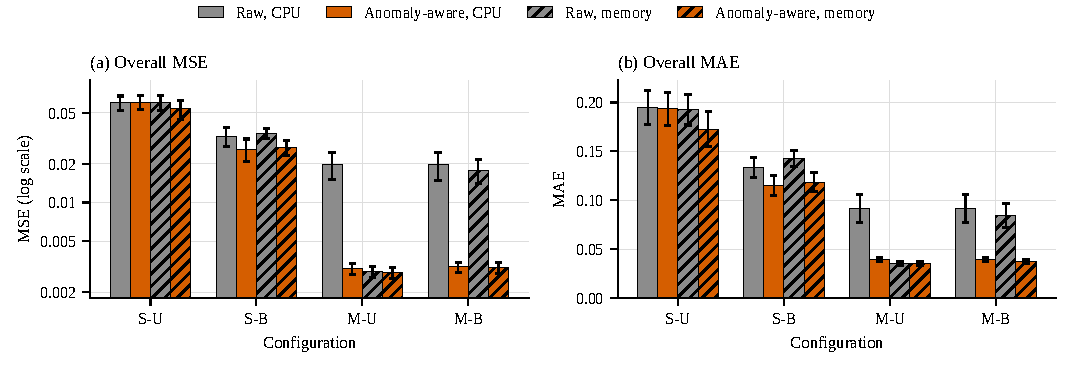
\includegraphics[width=\textwidth]{hbnn_fig_accuracy.pdf}
\caption{Overall MSE (a, log scale) and MAE (b) of the HBNN with raw inputs and with anomaly-aware inputs for the four configurations. Bars are means over 11 traces and 3 seeds; error bars show the standard error.}
\label{fig:hbnn_acc}
\end{figure*}

\begin{figure*}[!t]
\centering
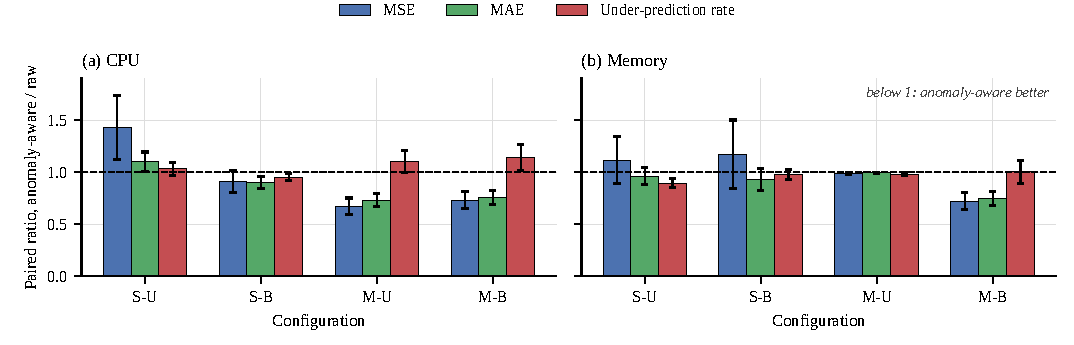
\includegraphics[width=\textwidth]{hbnn_fig_ratio.pdf}
\caption{Mean of the paired ratios anomaly-aware over raw, computed per matched trace and seed, for CPU (a) and memory (b). Values below one favour the anomaly-aware inputs. Error bars show the standard error of the 33 pairs.}
\label{fig:hbnn_ratio}
\end{figure*}

\begin{table}[!t]
\caption{Service-level behaviour of the HBNN upper bound (mean over CPU and memory, 11 traces, 3 seeds). SR is the realised success rate, TPR the total predicted resources as a percentage of actual demand, Cal.\ the mean absolute gap between realised and target SR over the four target levels, and Epist.\ the epistemic share of the total predictive variance.}
\label{tab:hbnn_service}
\centering
\footnotesize
\setlength{\tabcolsep}{3.6pt}
\begin{tabular}{llcccccc}
\toprule
 & & \multicolumn{2}{c}{95\% target} & \multicolumn{2}{c}{99\% target} & Cal. & Epist.\\
\cmidrule(lr){3-4}\cmidrule(lr){5-6}
Config. & Input & SR & TPR & SR & TPR & (pp) & (\%)\\
\midrule
S-U & Raw & 99.2 & 217.9 & 99.8 & 277.1 & 3.68 & 22.9\\
 & Anomaly & 99.1 & 231.8 & 99.8 & 296.3 & 3.73 & 26.2\\
\addlinespace[2pt]
S-B & Raw & 95.9 & 156.2 & 99.4 & 183.9 & 3.44 & 12.8\\
 & Anomaly & 95.6 & 150.6 & 99.1 & 175.7 & 3.59 & 16.7\\
\addlinespace[2pt]
M-U & Raw & 95.0 & 122.3 & 98.6 & 132.0 & 2.92 & 2.3\\
 & Anomaly & 95.8 & 115.6 & 98.5 & 121.9 & 1.87 & 3.4\\
\addlinespace[2pt]
M-B & Raw & 93.7 & 129.4 & 98.7 & 142.5 & 3.73 & 0.7\\
 & Anomaly & 95.8 & 116.4 & 98.4 & 123.0 & 2.15 & 5.7\\
\bottomrule
\end{tabular}
\end{table}

\begin{figure*}[!t]
\centering
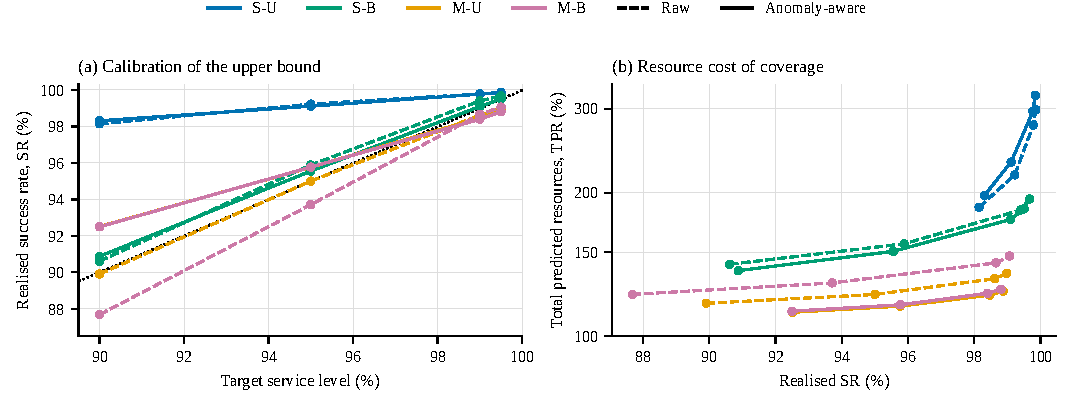
\includegraphics[width=\textwidth]{hbnn_fig_service.pdf}
\caption{Service-level behaviour of the HBNN upper bound, averaged over CPU and memory. (a) Realised success rate against the target service level; the dotted diagonal is perfect calibration. (b) Total predicted resources against realised SR, with a logarithmic vertical axis. Solid lines are anomaly-aware inputs, dashed lines raw inputs.}
\label{fig:hbnn_service}
\end{figure*}

\begin{figure*}[!t]
\centering
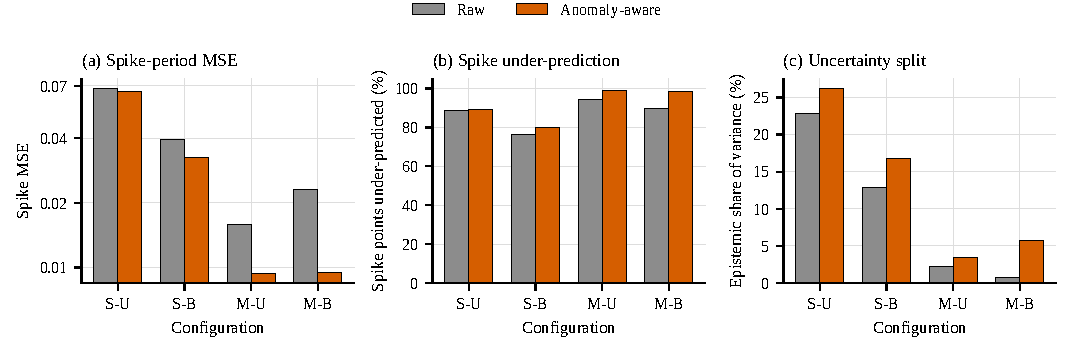
\includegraphics[width=\textwidth]{hbnn_fig_spike.pdf}
\caption{Spike-period behaviour and uncertainty of the HBNN, averaged over CPU and memory. (a) Spike MSE (log scale). (b) Share of spike points where the mean forecast lies below the actual demand. (c) Epistemic share of the total predictive variance.}
\label{fig:hbnn_spike}
\end{figure*}
